\section{Models}

We apply our methods to the following models:
\begin{itemize}
\item {\sc Imaginet}: A multi-modal GRU network which consists of two
  pathways, {\sc Visual} and {\sc Textual}, coupled via word
  embeddings.
\item {\sc LM}: A (unimodal) language model consisting of a Gated Recurrent
  Unit (GRU) network.
\item {\sc Sum}: A network with the same objective as the {\sc Visual}
  pathway of {\sc Imaginet}, but which uses sum of word embeddings
  instead of a GRU.
\end{itemize}
The rest of this sections gives more details for these models.

\subsection{Gated Recurrent Neural Networks}
\label{sec:gru}

One of the main difficulties for training traditional Elman networks
arises from the fact that they overwrite their hidden states at every
time step with a new value computed from the current input $x_{t}$ and
the previous hidden state $\mathbf{h_{t-1}}$. Similarly to LSTMs,
Gated Recurrent Unit networks introduce a mechanism which facilitates the retention of 
information over multiple time steps.
Specifically, the GRU computes the hidden state at current time step, $\mathbf{h}_{t}$, as the
linear combination of previous activation $\mathbf{h_{t-1}}$, and a new
{\it candidate} activation $\mathbf{\tilde{h}}_t$:
%
\vspace{-.2cm}
\begin{equation}
  \mathrm{GRU}(\mathbf{h}_{t-1}, \mathbf{x}_t) = (1 - \mathbf{z}_t)\odot \mathbf{h}_{t-1} + \mathbf{z}_t \odot \mathbf{\tilde{h}}_t
\vspace{-.1cm}
\end{equation}
%
where $\odot$ is elementwise multiplication, and the update gate
activation $\mathbf{z_{t}}$ determines the amount of new information
mixed in the current state:
%
\vspace{-.1cm}
\begin{equation}
\label{eq:gru-update}
   \mathbf{z}_t = \sigma_s(\mathbf{W}_z \mathbf{x}_t + \mathbf{U}_z \mathbf{h}_{t-1})
\vspace{-.1cm}
\end{equation}
%
The candidate activation is computed as:
%
\vspace{-.2cm}
\begin{equation}
\label{eq:gru-cand}
   \mathbf{\tilde{h}}_t = \sigma(\mathbf{W} \mathbf{x}_t + \mathbf{U}(\mathbf{r}_t \odot \mathbf{h}_{t-1}))
\vspace{-.1cm}
\end{equation}
%
The reset gate $\mathbf{r_{t}}$ determines how much of the current
input $\mathbf{x_{t}}$ is mixed in the previous state
$\mathbf{h}_{t-1}$ to form the candidate activation:
%
\vspace{-.2cm}
\begin{equation}
\label{eq:gru-reset}
   \mathbf{r}_t = \sigma_s(\mathbf{W}_r \mathbf{x}_t + \mathbf{U}_r \mathbf{h}_{t-1})
\vspace{-.1cm}
\end{equation}

% \iffalse
% \subsection{Sentiment Classifier}
% \label{sec:sentiment}
% \todo{Describe sentiment task and classifier in proper detail}

% For some of the experiments we trained a sentiment classifier on the
% Sentiment Tree-bank \cite{socher2013recursive} a widely used data set
% to test neural network models for natural-language processing. It is a
% phrase level sentiment classification data set containing sentiment
% labels for parse tree constituents, from sentences to word level, for
% 215,154 phrases in 11,855 sentences. We trained our sentiment
% classifier to perform the 5 level fine-grained (very positive,
% positive, neutral, negative and very negative) sentiment
% classification task. The input parse trees were flattened, by
% transforming each parse tree node into a sequence of tokens. Each
% token sequence of length $n$ is first mapped to hidden representations
% $h_{t_{0}}, \ldots, h_{t_{n}}$ and the last representation is fed into
% a softmax classifier layer to predict the final sentiment score. The
% architecture we used is a simple single layer Gated Recurrent Unit
% Network:

% \begin{enumerate}
% \item Embedding layer
% \item GRU layer with clipped rectified activation
% \item Softmax Output layer
% \end{enumerate}

% The model was trained with the Adam optimizer using mini-batches, $L_{2}$ regularization and no dropout. The number of hidden neurons and the dimensionality of the word embeddings was set to 50. 
% \fi

\subsection{Imaginet}
\label{sec:imaginet}



{\sc Imaginet} introduced in \namecite{chrupala2015learning} is a
multi-modal GRU network architecture that learns visually grounded
meaning representations from textual and visual input.  It acquires 
linguistic knowledge via comprehension and production, by receiving a
description of a scene and trying to visualise it through predicting a visual
representation for the textual description, while concurrently predicting 
the next word in the sequence. 

\begin{figure}
\begin{center}
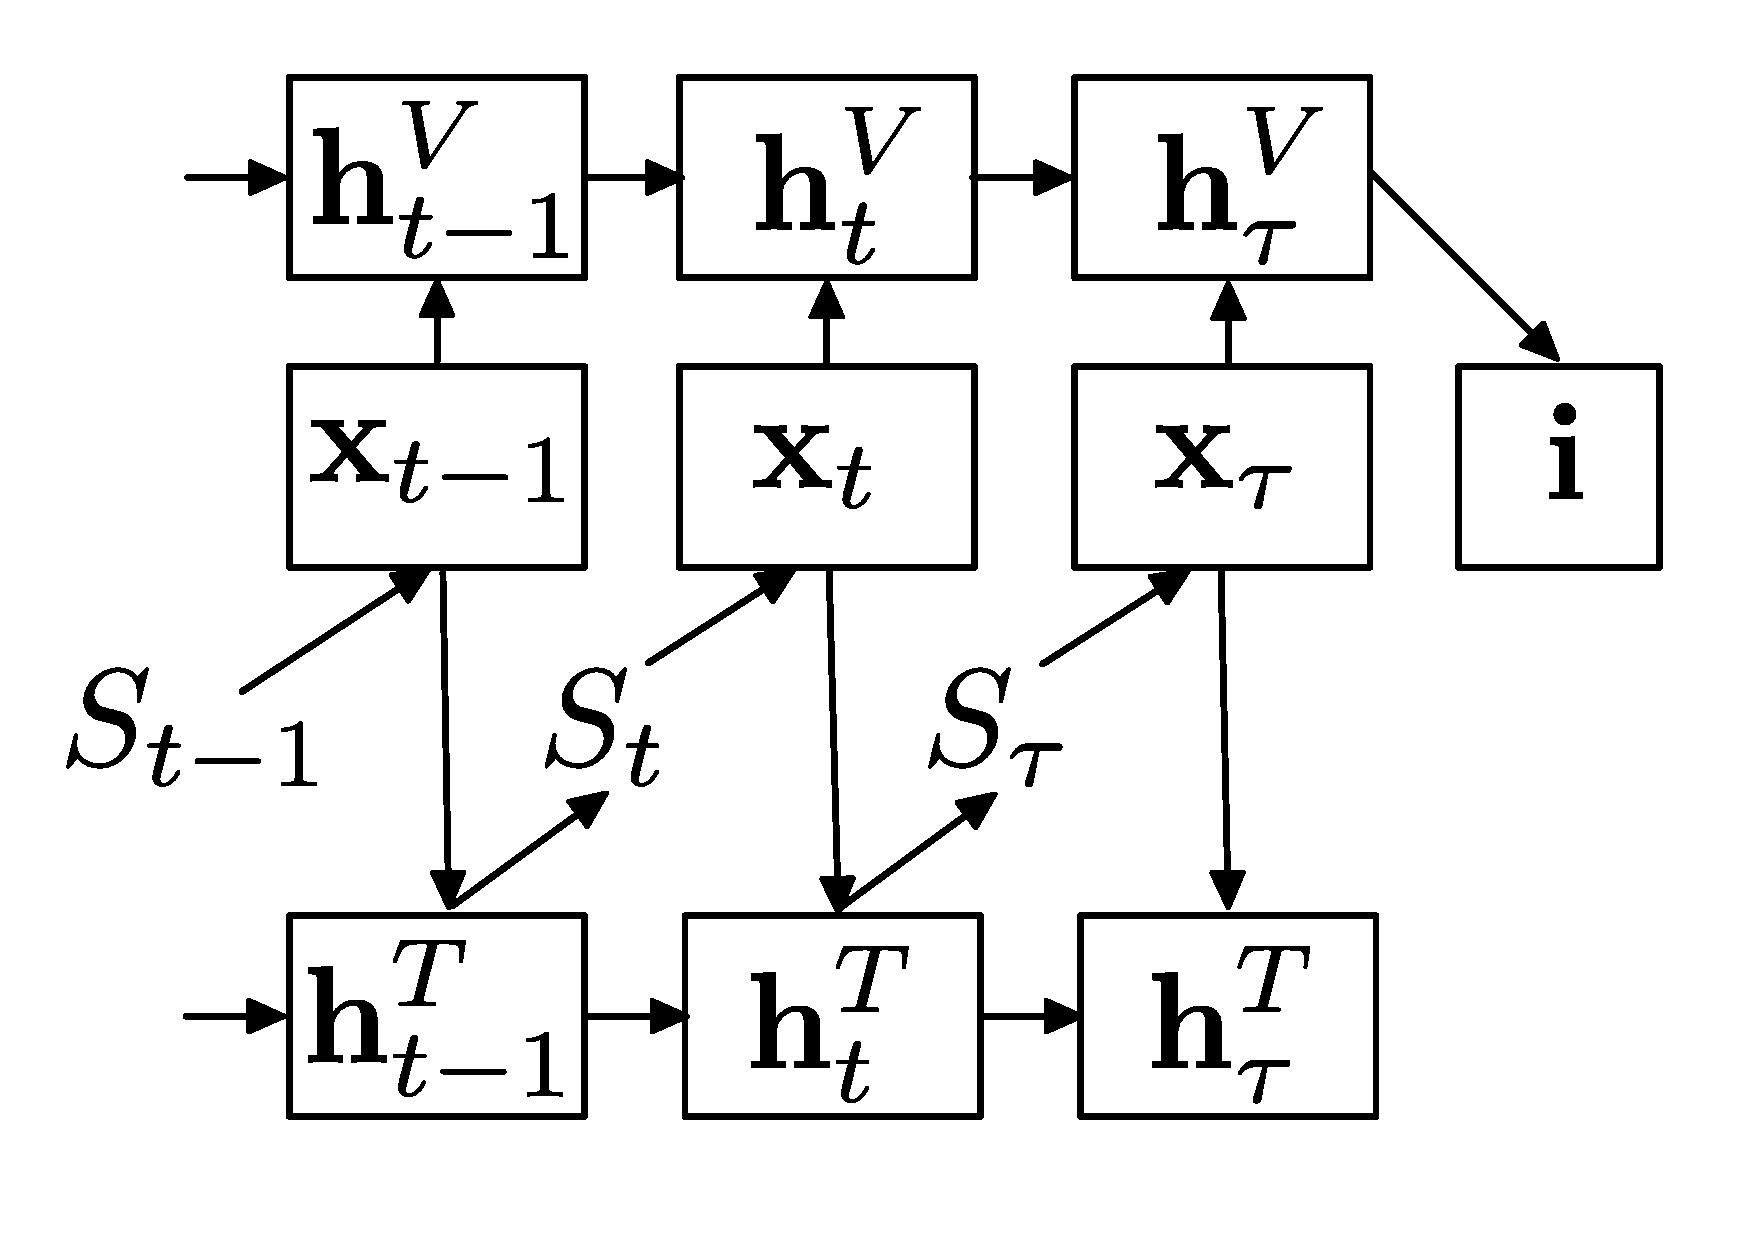
\includegraphics[scale=0.2]{imaginet.pdf} 
\caption{Structure of {\sc Imaginet}, adapted from \protect\cite{chrupala2015learning}.}
\label{fig:imaginet}
\end{center}
\end{figure}

Figure~\ref{fig:imaginet} shows the structure of {\sc Imaginet}. As can
be seen from the figure, the model consists of two GRU pathways, 
{\sc Textual} and {\sc Visual}, with a shared word-embedding matrix. 
The inputs to the model are pairs of image descriptions and their 
corresponding images. The {\sc Textual} pathway predicts the next 
word at each position in the sequence of words in each caption, whereas the 
{\sc Visual} pathway predicts a visual representation of the image that depicts the 
scene described by the caption after the final word is received.

Formally, each sentence is mapped to two sequences of hidden states, 
one by {\sc Visual} and the other by {\sc Textual}:
\vspace{-.2cm}
\begin{align}
  \mathbf{h}^{V}_t = \mathrm{GRU}^V(\mathbf{h}^{V}_{t-1},\mathbf{x}_t)\\
  \mathbf{h}^{T}_t = \mathrm{GRU}^T(\mathbf{h}^{T}_{t-1},\mathbf{x}_t)
\vspace{-.1cm}
\end{align}
%
At each time step {\sc Textual} predicts the next word in the sentence
$S$ from its current hidden state $\mathbf{h}^{T}_t$, while {\sc
  Visual} predicts the image-vector\footnote{Representing the full image, 
  extracted from the pre-trained Convolutional Neural Network of 
  \namecite{simonyan2014very}. \label{edit:dumdumeddy}}
$\hat{\mathbf{i}}$ from its last
hidden representation $\mathbf{h}^{V}_t$.
%
\vspace{-.2cm}
\begin{align}
   \hat{\mathbf{i}} &= \mathbf{V} \mathbf{h}^{V}_\tau \\
    p(S_{t+1}|S_{1:t}) &= \mathrm{softmax}(\mathbf{L}\mathbf{h}^T_t)
\vspace{-.1cm}
\end{align}
%
The loss function is a multi-task objective which penalizes error on
the visual and the textual targets simultaneously. The objective
combines cross-entropy loss $L^{T}$ for the word predictions
and cosine distance $L^V$ for the image
predictions.
%
%\vspace{-.2cm}
\begin{align}
%\begin{equation}
%\label{eq:lossce}
&L^{T}(\theta) = {-} \frac{1}{\tau}\sum_{t=1}^\tau \log p(S_t|S_{1:t}) \\
%\end{equation}
%
%\vspace{-.2cm}
%\begin{equation}
%\label{eq:losscos}
&L^V(\theta) =  1 - \frac{\hat{\mathbf{i}} \cdot \mathbf{i}}{\| \hat{\mathbf{i}} \| \| \mathbf{i} \|} \\
%\end{equation}
%
%\vspace{-.2cm}
%\begin{equation}
%\label{eq:losscombo}
&L = \alpha L^T + (1-\alpha)L^{V}
\end{align}
%L^V(\theta) &= \frac{1}{K}\sum_{k=1}^K(\hat{i}_k-i_k)^2
%

\noindent
For more details about the {\sc Imaginet} model and 
its performance see \namecite{chrupala2015learning}.

In our version of the model we add two minor modifications 
compared to the original {\sc Imaginet}. As the performance of
{\sc Visual} is measured on image-retrieval, which is based on cosine 
distances we use cosine distance as the visual loss.
Moreover, we observe that using standardized image vectors, where each dimension 
is transformed by subtracting the mean and dividing by standard deviation further
improves performance.


%\todo{should we include somewhere where the image representations are coming from?}
% The model achieves near state-of-the-art results on MS-COCO image
% retrieval and good performance on other natural language
% understanding tasks. For the detailed results and more information
% please consult

% he model performance was evaluated on the test on image-retrieval
% and paraphrase retrieval - we consider captions belonging to the
% same image as paraphrases. Image retrieval is performed by the {\sc
% Visual} pathway by projecting the validation captions to the image
% space and ranking the images according to there cosine similarity to
% the projection. The model achieves a performance of Recall@1=0.06,
% Recall@5=0.20 and Recall@10=0.29. The paraphrase retrieval task is
% performed using the last hidden states of {\sc Textual} or {\sc
% Visual} to represent the captions in the validation set. As
% demonstrated by Table \ref{tab:retrieval} the representations
% computed by {\sc Textual} captures the paraphrase relationship
% better in the particular setting.



\subsection{Unimodal language model}
The model {\sc LM} is a language model analogous to the {\sc Textual}
pathway of {\sc Imaginet} with the difference that its word embeddings
are not shared, and its loss functions is the cross-entropy on word
prediction. Using this model we remove the visual objective as a
factor, as the model does not use the images corresponding to captions
in any way.

\subsection{Sum of word embeddings}
The model {\sc Sum} is a stripped down version of the {\sc Visual}
pathway, which does not share word embeddings, only uses the cosine
loss function, and replaces the GRU network with a summation over word
embeddings. It this removes the effect of word order from
consideration. We use this model as a baseline in the sections which
focus on language structure. 
